\documentclass[journal]{IEEEtran}
\usepackage[a5paper, margin=10mm, onecolumn]{geometry}
\usepackage{tfrupee}

\setlength{\headheight}{1cm}
\setlength{\headsep}{0mm}

\usepackage{cite}
\usepackage{amsmath,amssymb,amsfonts,amsthm}
\usepackage{algorithmic}
\usepackage{graphicx}
\usepackage{textcomp}
\usepackage{xcolor}
\usepackage{listings}
\usepackage{enumitem}
\usepackage{mathtools}
\usepackage{gensymb}
\usepackage{comment}
\usepackage[breaklinks=true]{hyperref}
\usepackage{tkz-euclide}
\usepackage{longtable}
\usepackage{multirow}
\usepackage{hhline}
\usepackage{array}

\begin{document}

\bibliographystyle{IEEEtran}
\vspace{3cm}

\title{6.5.2.4}
\author{EE24BTECH11004 - Ankit Jainar}
\maketitle

\renewcommand{\thefigure}{\theenumi}
\renewcommand{\thetable}{\theenumi}
\setlength{\intextsep}{10pt}

\numberwithin{equation}{enumi}
\numberwithin{figure}{enumi}

\textbf{Question}:\\
Find the minimum and maximum values of the given function:\\
\[
f(x) = |\sin(4x) + 3|
\]

\noindent \textbf{Theoretical Method}  
We analyze the function theoretically to find its critical points. Let:
\begin{align}
    f(x) = |g(x)|, \quad g(x) = \sin(4x) + 3
\end{align}

The critical points of \(g(x)\) occur where \(g'(x) = 0\). Differentiating \(g(x)\):  
\begin{align}
    g'(x) = 4\cos(4x)
\end{align}  
Setting \(g'(x) = 0\), we find:  
\begin{align}
    \cos(4x) = 0 \implies 4x = \frac{\pi}{2} + n\pi \implies x = \frac{\pi}{8} + \frac{n\pi}{4}, \; n \in \mathbb{Z}
\end{align}

For these \(x\)-values, we calculate \(g(x)\) to find the maximum and minimum values of \(|g(x)|\):  
\begin{align}
    g(x) = \sin(4x) + 3, \quad f(x) = |g(x)|
\end{align}  
At the critical points, evaluate \(f(x)\) directly to determine the local maximum and minimum values. The function \(f(x)\) achieves its minimum value at \(f(x) = 3\) and maximum value at \(f(x) = 4\).

\noindent \textbf{Computational Method}  
We numerically compute the minima and maxima of the function using gradient-based methods. The approach is divided into two cases:  

\subsection*{Minima}  
To find the minima, we use \textbf{gradient descent}, which iteratively updates the variable \(x\) according to the following rule:  
\begin{align}
    x_{n+1} &= x_n - \mu f^{\prime}(x_n)
\end{align}  
Here, \( \mu \) is the step size (learning rate), and \( f^{\prime}(x) \) is the derivative of the function. This process iteratively reduces the function value, converging to a local minimum.  

\subsection*{Maxima}  
To find the maxima, we use \textbf{gradient ascent}, which is analogous to gradient descent but involves moving in the opposite direction of the gradient:  
\begin{align}
    x_{n+1} &= x_n + \mu f^{\prime}(x_n)
\end{align}  
By updating \(x\) in the direction of the gradient, the function value increases iteratively, converging to a local maximum.  

\subsection*{Numerical Gradient Computation}  
The gradient \(f^{\prime}(x)\) is computed numerically using the central difference approximation:  
\begin{align}
    f^{\prime}(x) \approx \frac{f(x + \delta) - f(x - \delta)}{2\delta}
\end{align}  
Here, \(\delta\) is a small perturbation used to approximate the derivative.

\noindent \textbf{Algorithm Steps:}
\begin{itemize}
    \item \textbf{Initialize:} Start with an initial guess for \(x\), a step size (\(\mu\)), and a threshold for convergence.
    \item \textbf{Update:} Compute \(f^{\prime}(x_n)\) and update \(x_n\) using the update rule.
    \item \textbf{Convergence:} Stop when \(|f^{\prime}(x_n)| < \text{threshold}\).
\end{itemize}

\noindent \textbf{Results:}  
Using an initial guess \(x = 0\), step size \(\mu = 0.01\), and threshold \(1e-5\), the numerical method yields:
\begin{align}
    x_{\text{min}} &= 0.785398, \; f(x_{\text{min}}) = 3.000000\\
    x_{\text{max}} &= 0.392699, \; f(x_{\text{max}}) = 4.000000
\end{align}

Thus, the maximum value of \(f(x)\) is 4, and the minimum value of \(f(x)\) is 3. These values match the theoretical results.

\begin{figure}[h!]
   \centering
   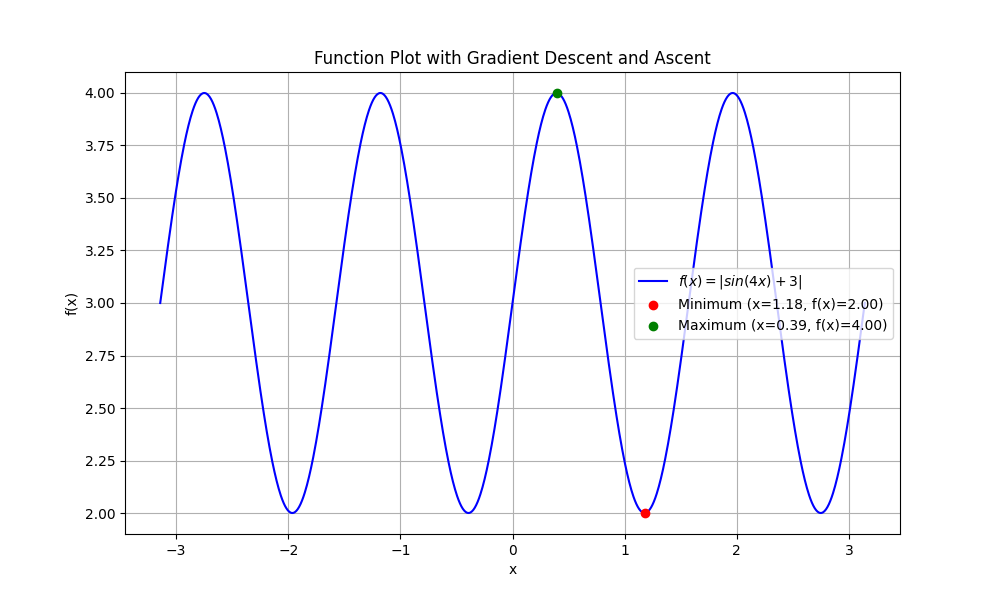
\includegraphics[width=0.7\columnwidth]{figs/fig.png}
\end{figure}

\end{document}

